\chapter{Implementierung}

In diesem Kapitel wird die Implementierung der Ingestion-Schnittstelle besprochen.
In \cref{fig:impl-arch} ist die Systemarchitektur zu sehen.
Diese zeigt alle Komponenten der Schnittstelle und wie diese interagieren.
In den folgenden Abschnitten wird deren Funktionsweise erklärt.
Dabei wird darauf eingegangen, welche Techniken angewendet wurden und warum diese gewählt wurden.
Bei den implementierten Mircoservices wird auch auf entwickelte Algorithmen und Vorgehensweisen eingegangen, mit den bestimmte Aufgaben gelöst werden.
Die Beschreibungen gehen dabei nicht zu sehr ins Detail.
Hier soll eher vermittelt werden, wie ein Problem gelöst wurde, unabhängig von gewählten Rahmenwerken oder Bibliotheken, solange diese nicht notwendig für die Lösung des Problems sind.
Für den API-, Ingestion- und Continuation-Service werden Konfigurationsdateien im YAML-Format\footnote{https://yaml.org/} verwendet.
Über diese werden Verbindungsinformationen und service-übergreifende Parameter konfiguriert.
Am Ende wird auch auf die Bereitstellung eingegangen.
Das heißt wie das fertige System gestartet und verwendet werden kann.


\begin{figure}
    \centering
    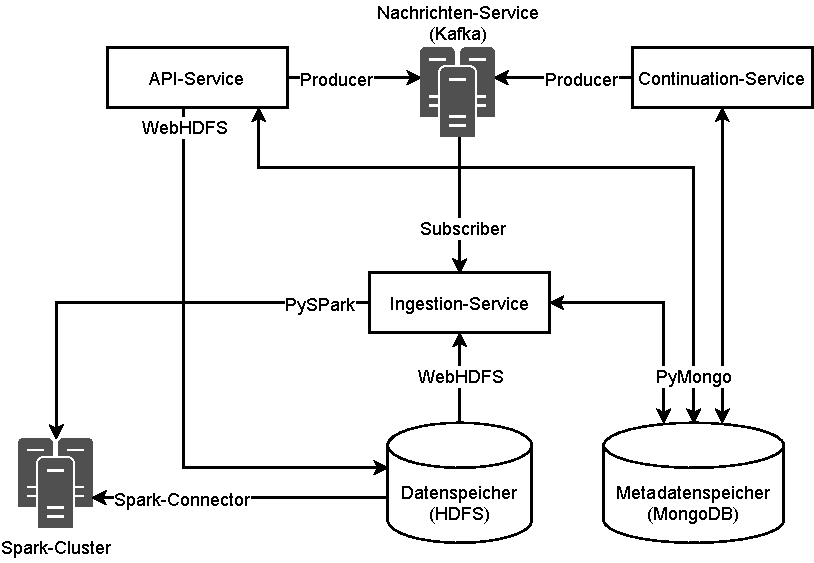
\includegraphics[height=8cm]{Grafiken/Umsetzung-System-Architektur.pdf}
    \caption{Implementierte Systemarchitektur}
    \label{fig:impl-arch}
\end{figure}

\section{Programmiersprache}

Durch die Verwendung von Apache Spark ist die Auswahl der Programmiersprachen auf Java, Python und Scala eingegrenzt.
Da der Prototyp in Python geschrieben wurde und dieser zum Api-Service erweitert werden soll, ist Python hierfür die Wahl.
Auch für die Implementierung des Ingestion-Service bietet Python einige Vorteile.


Bei der Verwendung von Java und Scala wird ein fertig kompiliert mit dem Befehl "`spark-submit"' zur Aufügrung an Spark gesendet.
Das bedeutet, dass der Code dieser Jobs bereits feststehen muss.
Neben dieser Option gibt es in Python auch die Möglichkeit, dass sich der Interpreter zur Laufzeit um die korrekte Ausführung der Jobs kümmert.
So ist es möglich ebenfalls für jede Anfrage speziell konifugrierte Jobs zu erstellen, die nicht vorher schon kompiliert sein müssen.
Das senkt die Komplexität bei der Entwicklung der Ingestion \parencite{pyspark-int}.

Auch für die Plugins hat Python einen Vorteil.
Man kann dynamisch Programmcode aus Dateien laden und inspizieren.
So können für jede Ausführung die Plugins einer Datenquelle frisch geladen werden.
Es muss nur dafür gesorgt werden, dass auch die Abhängigkeiten alle erfüllt sind.

Um die Entwicklung einheitlich zu halten, wird auch der Continuation-Service in Python implementiert.
\section{Nachrichtensystem}

Für die Übermittlung von Nachrichten zwischen verschiedenen Anwendungen gibt es sogenannte Message-Broker.
Diese koordinieren als Mittelsmann die Verteilung der Nachrichten an verschiedene Empfänger.
Das hat den Vorteil, dass der Sender unabhängig von den Empfängern wird und die Kommunikation asynchron statt finden kann \parencite{message-broker}.

Es gibt mittlerweile einige Projekte, diese Aufgabe auf verschiedene Arten lösen.
Hier wird dafür Apache Kafka verwendet, welches im Big Data Bereich weit verbreitet ist um Datenströme zu verarbeiten.
Daher macht es Sinn, dieses in das Data-Lake-System zu integrieren und darin bereit zu stellen.
Um das System dabei nicht unnötig komplex und zu groß werden zu lassen, wird daher auf einen anderen Message-Broker verzichtet.

Da Kafka ein Event-Streaming-System ist, wird ab hier nicht mehr vom Austausch von Nachtrichten, sondern von Events gesprochen.
Für diese Events müssen Topics zur Einordnung fetsgelegt werden.
Die Schlüssel sollten dabei so gewählt werden, dass Kafka auch für andere Datenströme verwendet werden kann, ohne, dass zu Konflikten kommt.
Daher werden die Topics der internen Kommunikation des Data-Lake-Systems immer mit "`dls\_\_"' als Prefix benannt werden.
Danach folgt der Bereich, den das Event betrifft, hier zum Beispiel "`ingestion"'.
An diesen Namen kann dann noch weiter Unterscheidung angehängt werden.
Für das Ausführen einer Ingestion wäre damit die Topic "`dls\_\_ingestion\_\_run"'.

Wenn mehrere Consumer in einer Gruppe für eine Topic sind, werden Events nicht an alle sondern immer nur an einen aus der Gruppe gesendet.
Dieser Mechanismus kann für den Lastausgleich an bestimmten Stellen verwendet werden.
Für die Ingestion kann so der Ingestion-Services einfach repliziert werden.
\section{Datenbank und Datenmodell}

Da das Datenmodell einer Datenquelle eine verschachtelte Struktur hat, bietet sich hier als einfachste Lösung die Verwendung einer Dokumenten-orientierten NoSQl-Datenbank an.
Das hat den Vorteil, dass diese Listen direkt in den Objekten der Datenquellen abgelegt werden können.
In relationalen Datenbanken, die Tabellen verwenden, müsste man für jedes Modell eine eigene Tabelle erstellen und die Verknüpfungen über über JOIN-Operationen auflösen.
Bei jeder Abfrage einer Datenquelle werden die verknüpften Einträge der Ingestion-Events oder Revisionen gebraucht, was somit zu einem größeren Aufwand führt.
Außerdem gibt es viele Anfragen auf die Datenquellen, da diese nicht zwischen den Mircoservices ausgetauscht werden und so nicht im Speicher vom Service verwaltet werden können.
Daher ist es effizienter die relevanten Daten direkt mit einer Abfrage laden zu können.
Hier kommt MongoDB\footnote{https://www.mongodb.com/} als Datenbank zum Einsatz.
MongoDB kann frei verwendet werden und bei bei größeren Datenmengen verteilt eingesetzt werden.

\section{Datenspeicher}

Für das Speichern von Daten mit einer Versionierung ist Delta Lake eine gut gepflegte und in Spark integrierte Lösung.
Neben den versionierten müssen auch Daten mit und ohne Struktur gespeichert werden.
Für strukturierte und semistrukturierte Daten kommt das Parquet-Format zum Einsatz.
Unstrukturierte Daten werden im ursprünglichen Format im HDFS abgelegt.

Als Speicher wird das HDFS verwendet.
In diesem können sowohl die Delta Tabellen als auch andere Parquet-, Quell- und Plugin-Dateien abgelegt werden.
Alle Microservices haben über die WebHDFS-Schnittstelle Zugriff auf die Daten.
Im HDFS wird eine Verzeichnisstruktur (\cref{fig:hdfs-folder}) für alle Daten des Data Lakes angelegt.
Diese geht von dem Ordner "`datalake"' aus, der im Root-Verzeichnis des HDFS angelegt wird.
In diesem Ordner werden die Unterordner
\begin{itemize}
    \item "`sources"' für Quell-Dateien,
    \item "`plugins"' für Plugin-Dateien und
    \item "`data"' für die Ablage von geladenen Daten erstellt.
\end{itemize}

In den Ordnern "`sources"' und "`plugins"' werden dann für jede Datenquelle Ordner mit deren Id angelegt, in denen die hochgeladenen Dateien abgelegt werden.

Für die geladenen Daten werden die Ordner \begin{itemize}
    \item "`structured"' für semi-/strukturierte Daten ohne Versionierung,
    \item "`unstructured"' für unstrukturierte Daten und 
    \item "`delta"' für semi-/strukturierte Daten mit Versionierung.
\end{itemize}
innerhalb des Ordners "`data"' angelegt.
Diese unterteilen sich dann ebenfalls wieder in Ordner für jede Datenquelle mit der Id als Name.

\begin{figure}
    \centering
    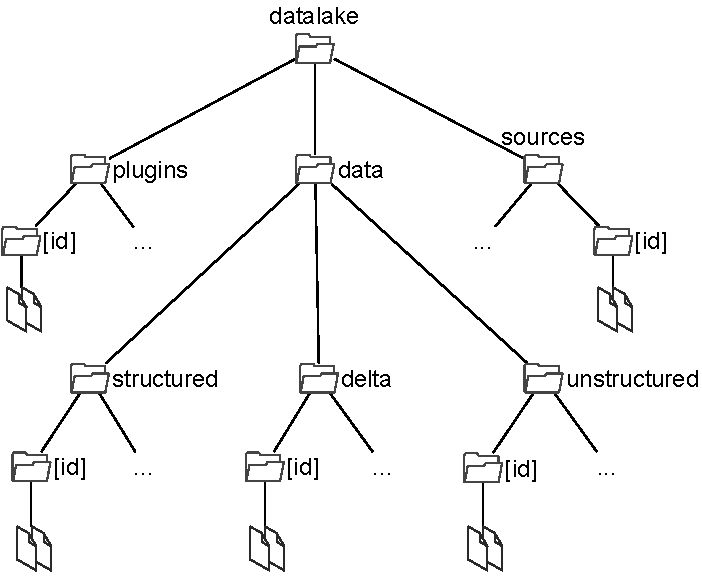
\includegraphics[width=.6\textwidth]{Grafiken/Umsetzung-Verzeichnisse.pdf}
    \caption{HDFS Verzeichnisstruktur}
    \label{fig:hdfs-folder}
\end{figure}
\section{API-Service}

Bei HTTP-Anfragen können Inhalte in der Anfrage als verschiedene Typen übergeben werden.
Hier wird der Typ \verb|mutltipart/forma-data| verwendet.
Bei diesem Typ können sowohl Text als auch Dateien übertragen werden.
Jeder Text oder jede Datei werden dabei als Wert betrachtet und müssen einen Schlüssel vergeben bekommen.
Das heißt, dass alle Informationen als Schlüssel-Wert-Paar an den API-Service gesendet werden.
Die Schlüssel, die verwendet werden sollen, werden wie folgt vergeben.
Die DatasourceDefinition bekommt den Schlüssel "`datasource-definition"'.
Der Wert dahinter kann entweder eine JSON-Datei oder ein JSON-Text sein.
Die Schlüssel der hochgeladenen Dateien sind frei wählbar.

Die DatasourceDefinition besteht zu Teilen aus Feldern, die automatisch durch die Services gefüllt werden.
Daher wird ein weiteres Datenmodell für die Eingabe von Informationen bei der REST-API benötigt.
Dafür wird die DatasourceDefinitionInput (\cref{fig:datasource-definition-input}) verwendet.
In diesem Modell befinden sich alle Felder, die durch den Benutzer befüllt werden können.
Aus den Daten dieses Modells erstellt der API-Service dann die Revisionen für die DatasourceDefinition.

\begin{figure}
    \centering
    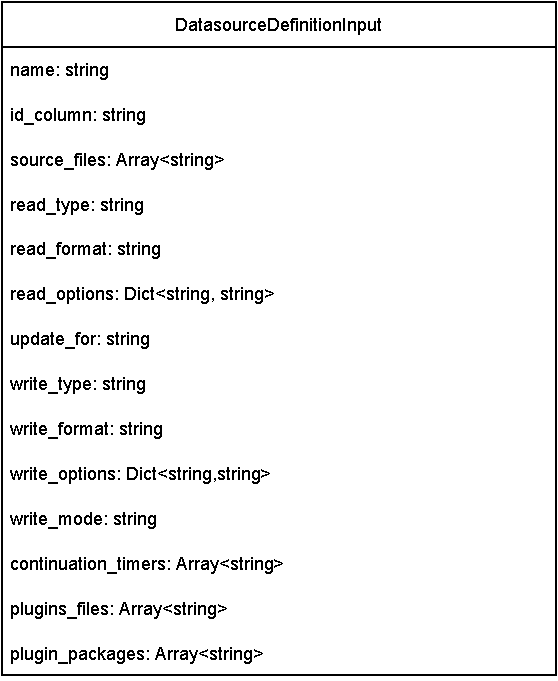
\includegraphics[width=.65\textwidth]{Grafiken/Umsetzung-Definition-Input.pdf}
    \caption{Felder Datenquellen-Eingabe}
    \label{fig:datasource-definition-input}
\end{figure}

\subsection{Hochladen von Dateien}

Für jede Datenquelle können Quell- oder Plugin-Dateien hochgeladen werden.
Um eine hochgeladene Datei in der Datenquelle auch zu verwenden, muss der Schlüssel, unter dem die Datei hochgeladen wird, in der entsprechenden Liste entweder unter "`source\_files"' oder unter "`plugin\_files"' hinzugefügt werden.
Alternativ können auch die Namen unter denen bereits Dateien für die Datenquelle gespeichert wurden in die Listen eingefügt werden.

Bei der Verarbeitung der Eingabe prüft der API-Service für jeden Eintrag der Listen, ob eine Datei mit diesem Schlüssel hochgeladen wurde.
Ist das der Fall, wird die entsprechende Datei in das HDFS hochgeladen.
Der Name, unter dem die Datei gespeichert wird, setzt sich aus der Nummer der Revision, dem vergebenen Schlüssel und der Endung der Datei zusammen.
Lädt man also eine bei der ersten Erstellung einer DatasourceDefinition eine Datei "`data.json"' mit den Schlüssel "`file"' hoch, wird diese als "`r000\_file.json"' im "`sources"'-Ordner der DarasourceDefinition gespeichert.
Analog werden Plugin-Dateien genauso behandelt.

Wenn keine Datei in der Anfrage gefunden wurde, wird geschaut, ob im HDFS eine Datei mit dem Namen existiert.
Wird eine Datei gefunden, wird der Name an die neue Revision angehangen.
Es ist wichtig zu beachten, dass alle Dateien der alten Revision, die nicht explizit in einer der Listen angegeben werden, nicht in der neuen Revision verwendet werden.
Sie bleiben jedoch gespeichert und können später wieder hinzugefügt werden.
Da die Dateien nach den Datenquellen aufgeteilt sind, ist es aktuell nicht möglich Plugins oder Quell-Dateien in anderen Datenquellen wieder zu verwenden.
Hier müsste man die Datei für jede Datenquelle hochladen.

\section{Continuation-Service}

Der Continuation-Service führt durchgehend eine Schleife zum Überprüfen der Datenquellen aus.
Bei der Prüfung wird immer der Status des aktuellsten IngestionEvent betrachtet.
Je nach Datenquelle wird dann entschieden, ob eine Ingestion gestartet werden soll.
Die Logik der Schleife besteht aus drei Teilen, wovon zwei die Datenquellen prüfen und einer die Zeit steuert, nachdem die Schleife erneut ausgeführt wird (\cref{algo:ci-loop}).
Das soll nur maximal jede Minute geschehen, da auch keine schnellere Ausführung über die Timer definiert werden kann.

Im ersten Teil werden alle Datenquellen einer Datenstrom-Ingestion kontrolliert.
Für diese wird eine neue Ingestion gestartet, wenn der Status "`FINISHED"' ist.
Der Status "`STOPPED"' bedeutet, dass die Ausführung mit Absicht beendet wurde und manuell gestartet werden muss.

Der zweite Teil überprüft alle Datenquellen, bei denen ein oder mehrere Timer gesetzt wurden.
Wenn der Status des letzten IngestionEvents nicht "`STOPPED"' oder "`FINISHED"' ist, wird die Überprüfung dieser Quelle abgebrochen.
Ansonsten wird jeder Timer mit dem aktuellen Zeitpunkt verglichen.
Hier wird die Methode $is_now$ verwendet.
Sie wird durch eine Python-Bibliothek bereitgestellt und prüft ob ein Cron-Timer, die auch für die kontinuierliche Ingestion eingesetzt werden, zum aktuellen Zeitpunkt zutrifft.
Trifft der Timer zu, wird eine Ingestion für die Datenquelle gestartet und sofort die nächste Datenquelle überprüft.

Der dritte Teil kontrolliert die Ausführungshäufigkeit.
Dazu wird am Anfang der Schleife der Startzeitpunkt gespeichert.
Nachdem alle Überprüfungen beendet wurden, wird auch der Endzeitpunkt gespeichert.
Wenn die Differenz der beiden geringer ist als eine Minute, wird die Schleife für die Dauer der Differenz angehalten.
Damit ist sichergestellt, das sie nicht häufiger als einmal pro Minute ausgeführt wird.

\begin{algorithm}
    \caption{Continuation loop}
    \label{algo:ci-loop}
    
    \KwData{-}
    \KwResult{-}
    
    $loopStart \gets$ current\_time() \;
    
    $streams \gets$ all\_datasource\_definition\_of\_type\_stream() \;
    \ForAll {$definition$ in $streams$} {
        $event \gets definition.last\_ingestion$ \;
        \If {$event.state$ is FINISHED} {
            publish\_run\_event\_for($definition.id$) \;
        }
    }
    
    $timed \gets$ all\_datasource\_definitions\_with\_timers() \;
    \ForAll {$definition$ in $timed$} {
        $event \gets definition.last\_ingestion$ \;
        $timers \gets definition.revision.continuation\_timers$  \;
        \If {$event.state$ is STOPPED or FINISHED} {
            \ForAll {$timer$ in $timers$} {
                \If {is\_now($timer$)} {
                    publish\_run\_event\_for($definition.id$) \;
                    \textbf{break}
                }
            }
        }
    }

    $loopEnd \gets$ current\_time() \;
    $loopDuration \gets loopEnd - loopStart$ \;
    \If {$loopDuration < 60$} {
        sleep($60 - loopDuration$) \;
    }

\end{algorithm}


\section{Ingestion-Service}

Wie in \fref{sec:entw-ingestion} beschrieben, wird für ein Event ein Prozess gestartet.
Der Name der Topic des Events zum Starten einer Ingestion ist "`dls\_\_ingestion\_\_run"'.
In \fref{sec:ingestion-run} wird der detailliere Ablauf mit den verschiedenen Wegen für Read- und SaveTypes beschrieben.
Vorher werden die benötigt Grundlagen zur Ausführung erläutert.

\subsection{Berechnen und Speichern der Änderungsdaten}
Um Änderungen in eine Delta Tabelle zu übernehmen, müssen die Änderungsdaten in einem Format sein, dass Aufschluss darüber gibt, welche Daten hinzugefügt, welche geändert und welche gelöscht worden sind.
Das hier verwendete Format muss genau dem gleichen Schema entsprechen, wie die original Daten.
Zusätzlich soll eine Spalte oder ein Feld auf der obersten Eben mit dem Namen "`cd\_deleted"' vorhanden sein.
Es enthält einen Boolean-Wert, der sagt, ob der Eintrag aus den Daten gelöscht wurde oder nicht.
Der Datensatz mit den Änderungsdaten darf außerdem nur geänderte Daten enthalten.
Aus diesem Format können, wie später gezeigt, die drei Operationen abgeleitet werden.

Um nicht auf ein externes Change-Data-Capture-System angewiesen zu sein, gibt es eine interne Lösung, die auf alle (semi-)strukturierten Daten angewendet werden kann.
Der \cref{algo:delta-calc} zeigt, wie aus zwei DataFrames die Änderungsdaten erzeugt werden.
Als Eingabe werden ein linkes DataFrame, mit dem aktuellen internen Stand, eine rechtes DataFrame, mit den neuen Daten und der Name der Id-Spalte benötigt.
Das Ergebnis ist ein DataFrame mit allen aktualisierten Datensätzen.
Es hat das gleiche Schema wie die Ursprungsdaten, aber mit der zusätzlichen Spalte, die Auskunft darüber gibt, ob ein Datensatz gelöscht wurde.

\begin{algorithm}
    \caption{Deltaberechnung}
    \label{algo:delta-calc}
    \KwData{leftDataFrame, rightDataFrame, idColumn}
    \KwResult{changeDataFrame}
    $leftDataFrame \gets$ add column with row hash \;
    $leftDataFrame \gets$ prefix column names with "`left\_"' \;
    $rightDataFrame \gets$ add column with row hash \;
    $rightDataFrame \gets$ prefix columnnames with "`right\_"' \;

    $changeDataFrame \gets$ full join over $idColumn$ of $leftDataFrame$ and $rightDataFrame$ \;

    $changeDataFrame \gets$ remove all rows where $left\_hash$ equals $right\_hash$ \;

    $changeDataFrame \gets$ remove hash columns

    $changeDataFrame \gets$ add row $cd\_deleted$ \;
    \eIf{$right\_idColumn$ is $null$}{$cd\_deleted = true$}{$cd\_deleted = false$}

    $changeDataFrame \gets$ merge left and right $idColumn$ into one $idColumn$
    \eIf{$left\_idColumn$ is not $null$}{$idColumn = left\_idColumn$}{$idColun = right\_idColumn$}

    $changeDataFrame \gets$ merge remaining columns with left and right value by always taking the right and removing prefix

\end{algorithm}

Das Einpflegen der Änderungen wird über die Delta Lake API gelöst.
Dazu werden die Änderungsdaten mit den aktuellen Daten über die Id-Spalte zusammengeführt.
Dabei können verschieden Fälle definiert werden.
Wenn die Ids einer Zeile gleich sind und die Spalte "`cd\_deleted"' $true$ enthält, wird die Zeile aus den Daten gelöscht, ansonsten wird der Datensatz aktualisiert.
Wenn die Ids nicht übereinstimmen und die Spalte "`cd\_deleted'" $false$ ist, dir der Datensatz als neue Zeile eingefügt.

\subsection{Plugins verwalten}
Für jede Ingestion wird auf dem Speichersystem des Mircoservices ein temporärer Ordner angelegt, in den die Plugins und deren Abhängigkeiten installiert werden.
Nach der Installation wird noch eine Datei angelegt, die für alle Pakete die Versionen enthält.
Das dient dazu, bei einer erneuten Ausführung auf dem Service nicht alle Pakete neu installieren zu müssen, sondern nur die mit geänderten Version.
Das beschleunigt die Ausführung der Ingestion.
Zum Schluss wird der Ordner, in den die Pakete installiert wurden an den Python-Pfad mit angehangen.
Damit wird dieser während der Ausführung manipuliert und die Pakete sind verfügbar.
Da jede Ingestion in einem eigenen Prozess beeinflussen die Änderungen an dem Python-Pfad den Ingestion-Service oder andere Prozesse nicht.

Im zweiten Schritt wird jede Python-Datei im Pluginordner als Modul geladen.
Die im Modul verfügbaren Methoden werden dann überprüft, ob sie auf eine Definition der möglichen Plugins passen.
Dazu wird der \fref{algo:check-method} verwendet.
Diesem werden das geladene Modul, ein Name der Methode, ein optionaler Rückgabetyp der Methode und eine Liste von Parameter, bei denen Name und Typ definiert ist.
Zur Überprüfung können alle Methoden in dem Modul auf ihren Namen geprüft werden.
Wenn eine Methode gefunden wurde, wird eine Signatur erzeugt und mit der übergebenen Definition verglichen.
Das Ergebnis sagt dann, ob diese Methode ein Plugin ist oder nicht.

Jedes geladene Modul wird auf Load- oder AfterLoad-Methoden geprüft.
Eine gefundene Load-Methode überschreibt immer die letzte gefunden, da bei einer Ausführung auch das Ergebnis dieser Methoden überschrieben werden würde.
Die AfterLoad-Methoden dagegen werden in einer Liste gespeichert.


\begin{algorithm}
    \caption{Pluginmethode überprüfen}
    \label{algo:check-method}

    \KwData{$plugin$, $name$, $return\_type$, $parameters$}

    \KwResult{$matches$}

    \If{plugin has NOT method with name $name$}{
        \Return{false}
    }

    $signature \gets$ signature of mehtod $name$

    \If{$return\_type$ is given AND $signature$ NOT returns type of $return\_type$}{
        \Return{false}
    }

    \ForAll{$param$ in $parameters$}{
        \If{$signature$ has NOT a parameter named $param.name$}{
            \Return{false}
        }

        \If{$signature$ type of parameter $param.name$ is NOT $parameter.type$}{
            \Return{false}
        }
    }

    \Return{true}

\end{algorithm}

\subsection{Ausführung der Ingestion}
\label{sec:ingestion-run}
Die Ausführung startet mit der Initialisierung, die die für die Ingestion benötigte Daten lädt.
Das ist zum Beispiel die DatasourceDefinition zu der Id aus den Events.
Danach wird entschieden ob eine Ingestion über Spark notwendig ist.
Hier spielt der Lesetyp eine große Rolle.
Eine Ingestion von Datendateien benötigt keine Spark, es werden einfach direkt die Dateien in das entsprechende Zielverzeichnis kopiert.
Für alle anderen Typen wird im nächsten Schritt die Ingestion vorbereitet.
Es werden die Plugins aus dem HDFS geladen und eine SparkSession erstellt.
Das Laden der Daten in ein DataFrame geschieht anschließend entweder über ein Plugin in oder das Standardvorgehen.
Falls auch After-Load-Plugins vorhanden sind werden diese ausgeführt.
Für die geladenen Daten wird dann entschieden, ob es sich um Änderungsdaten handelt oder welche berechnet werden müssen.
Je nach Schreib-Typ werden dann die Daten beziehungsweise Ändeurngsdaten gespeichert.
Für Datenströme wird am Ende noch ein Hintergrund Task gestartet, der auf Kafka Events zum stoppen dieser Ingestion wartet.
Hierfür wird die Topic "`dls\_\_ingestion\_\_stop\_ingestion"' mit der Id als Wert verwendet.
Wenn die Ingestion beendet wurde, wird zum Schluss die SparkSession gestoppt.

\begin{figure}
    \centering
    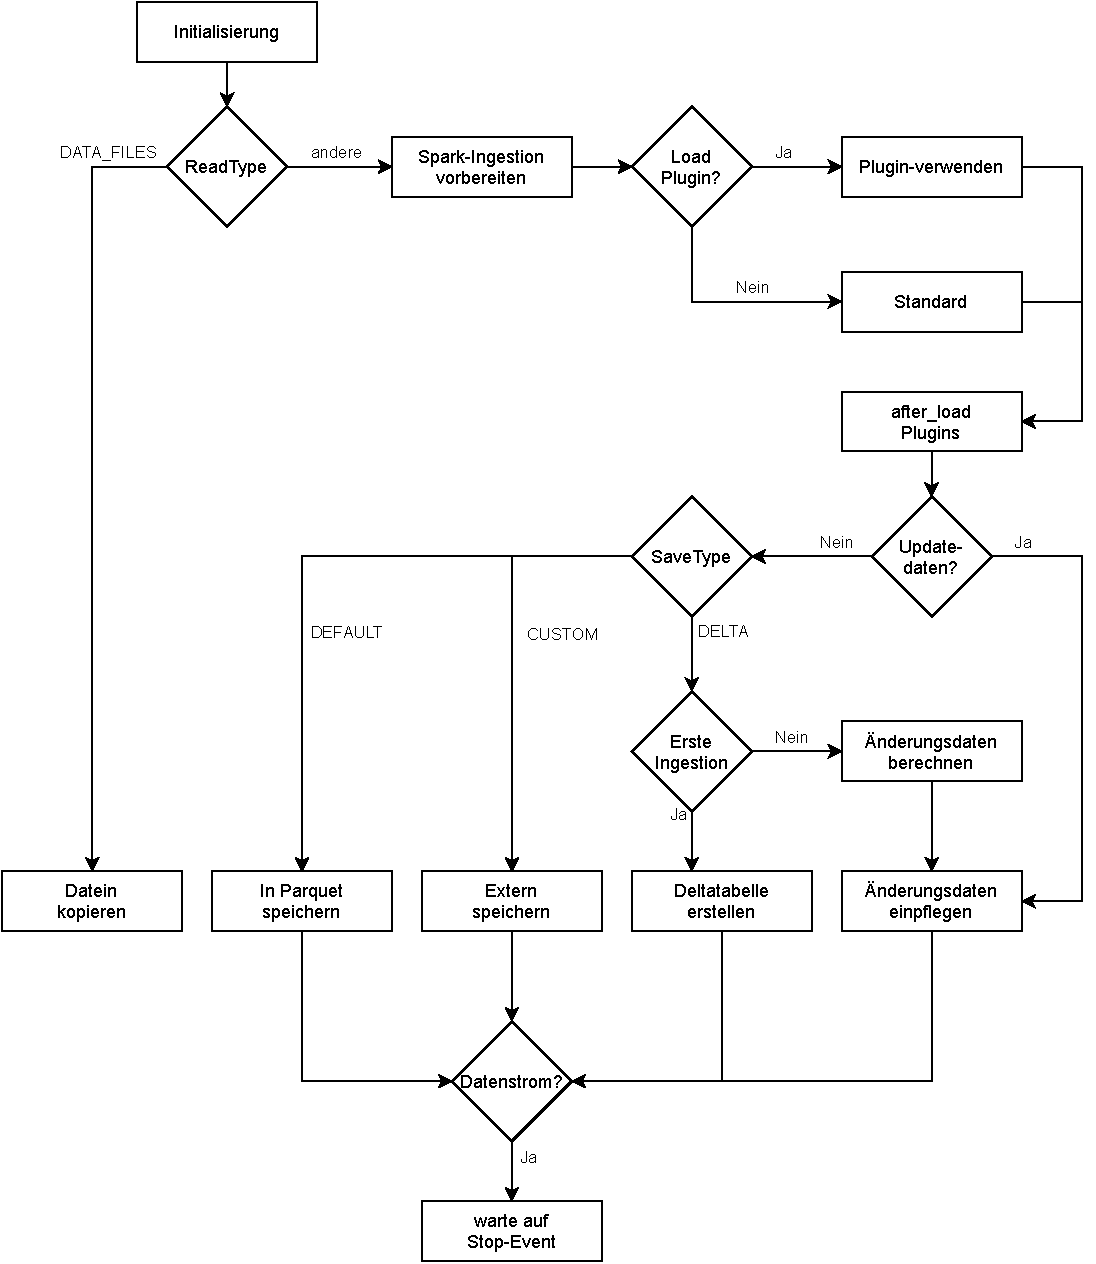
\includegraphics[width=\textwidth]{Grafiken/Umsetzung-Ingestion-Ablauf.pdf}
    \caption{Ablauf einer Ingestion}
    \label{fig:umsetz-ingestion-ablauf}
\end{figure}
\section{Bereitstellung}

Bei der Bereitstellung des gesamten Systems gibt es einen wichtigen Punkt der beachtet werden muss.
Viele der eingesetzten Services funktionieren als Cluster und benötigen mehrere Server um ausgeführt zu werden.
Nicht jede Umgebung kann diese Anzahl an Servern bereitstellen.
Daher müssen diese virtualisiert werden.
Dazu wird hier Docker\footnote{https://docker.com} verwendet.
Docker ist eine Laufzeit für Container.
Diese sind ähnlich zu klassischen virtuellen Maschinen, verbrauchen aber weniger Ressourcen.
Ein weiterer Vorteil ist, dass Container für bestimmte Anwendungen gebaut werden.
Ist ein Container einmal gebaut, kann er einfach verteilt und gestartet werden und ist direkt in einem lauffähigen Zustand.
Zum Beispiel gibt es fertige Container, um einen Spark-Master oder -Worker zu starten.
Damit ist der Aufbau eines Spark-Clusters wesentlich einfach und reproduzierbarer als die Installation in mehreren virtuellen Maschinen.
Zusätzlich gibt es Projekte, wie Kubernetes\footnote{https://kubernetes.io/} oder Docker Swarm\footnote{https://docs.docker.com/engine/swarm/}, die es erlauben Container auf einem verteilten Cluster auszuführen.
Diese werden dann über das Cluster verteilt und über ein virtuelles Netzwerk verbunden.
So wird auch die horizontale Skalierung der verfügbaren Hardware vereinfacht.

Das Ziel ist es, den gesamten Data Lake in Containern bereit zu stellen.
Dabei treten allerdings ein paar Hürden auf, da die verwendeten Rahmenwerke nicht alle auf die Verwendung in Containern ausgelegt sind.
Als erstes muss darauf geachtet werden, dass Container von sich aus keine Persistenz besitzen.
Den Daten, die nicht bei einem Neustart verloren gehen dürfen, müssen Volumes\footnote{https://docs.docker.com/storage/volumes/} zugeordnet werden.
Außerdem müssen alle Container im selben Netzwerk sein, damit diese untereinander Kommunizieren können.
Da die IP-Adressen, die die Container in diesen Netzwerken bekommen, nicht außerhalb des Netzwerks erreichbar sind, müssen sowohl das HDFS als auch die SparkSession so konfiguriert werden, dass sie die Host-Namen der Name- und DataNodes verwenden.
Die Host-Namen müssen dann auf die IP-Adresse des Servers aufgelöst werden, auf dem die Container laufen.
Um die Services in den Containern von außen erreichen zu können, müssen die verwendeten Ports freigegeben werden.
Dafür können Ports des Host-Systems zu Ports innerhalb des Containers zugeordnet werden.
Dabei darf ein Host-Port immer nur einmal verwendet werden.

Die Bereitstellung der Services in Docker erfordert den Bau eigener Container.
Als Basis wird das Docker-Image von Python verwendet.
Für jeden Service müssen alle Python-Quell-Dateien kopiert werden.
Bei der Ausführung ist es noch notwendig einen Ordner mit Konfigurationsdateien als Volume in den Container ein zu binden.

\subsection{Verwendete Docker Container}

In \cref{fig:docker-datalake} ist ein Beispiel zu sehen, welche Container für ein Data-Lake-System benötigt werden, wie es das Ergebnis dieser Arbeit ist.
Jeder Block repräsentiert einen Container.
Beschrieben werden hier nur die verwendeten Docker-Images und die freigegebenen Ports.
Der erste Port ist der Host-Port und der zweite der Ziel-Port im Container, die gleiche Notation wie sie von Docker benutzt wird.
Die restliche Konfiguration wird auf Grund der Übersichtlichkeit nicht gezeigt.
Alle Container liegen in dem gleichen Docker-Netzwerk.
Die grau hinterlegten Gruppen dienen nur der Verdeutlichung der Cluster.
Die Anzahl der Spark-Worker, DataNodes oder Kafka-Broker kann je nach Hardware-Ressourcen angepasst werden.
Alle Container bei denen der Docker-Image-Name mit "`datalake/"' beginnt sind selber für den Data Lake gebaut.
Das Docker-Image "`datalake/spark"' basiert auf "`bitnami/spark"' und wurde angepasst, die gleiche Python-Version zu verwenden, die auch bei den Services zum Einsatz kommt.

\begin{figure}
    \centering
    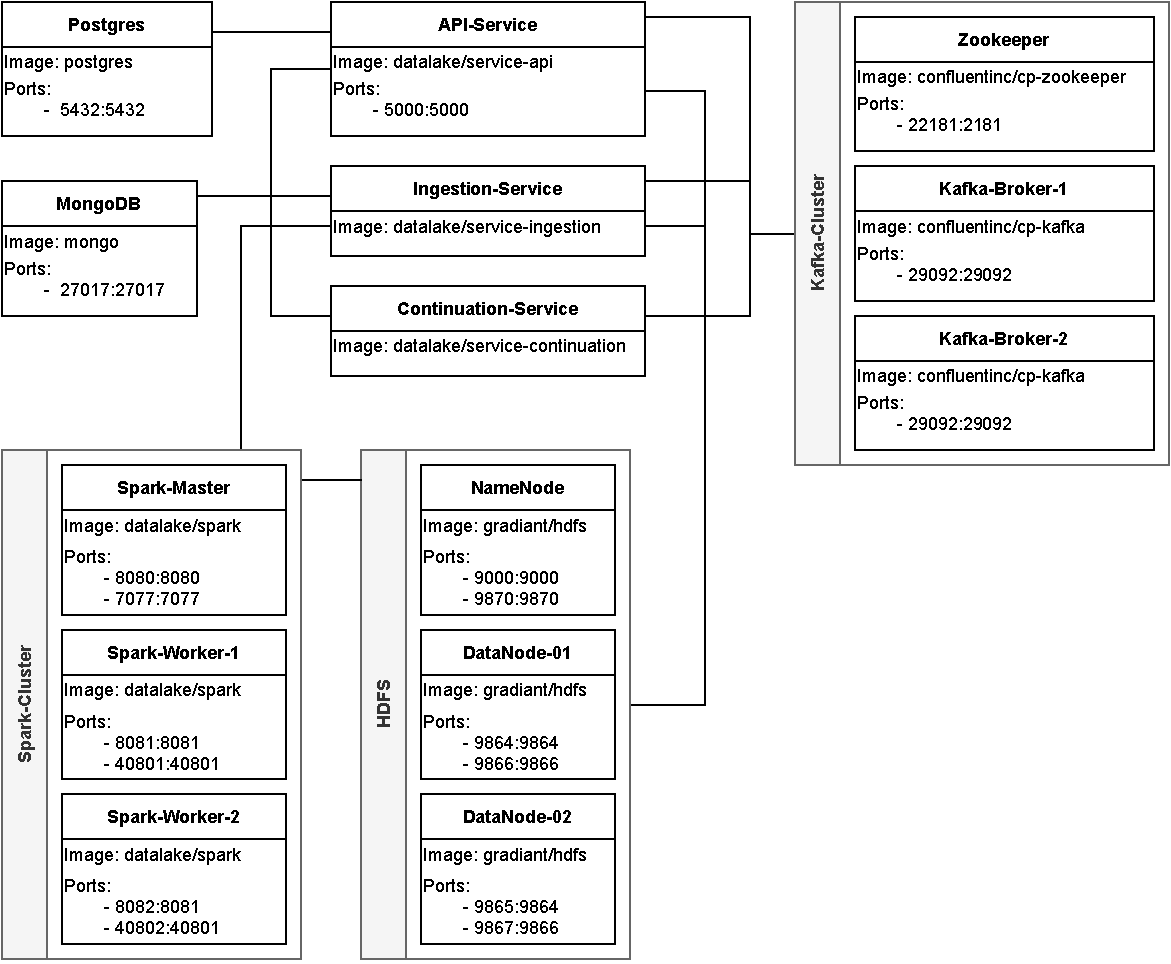
\includegraphics[width=\textwidth]{Grafiken/Umsetzung-Docker-Lake.pdf}
    \caption{Docker-Container für den Data Lake}
    \label{fig:docker-datalake}
\end{figure}
